% This is part of Un soupçon de mathématique sans être agressif pour autant
% Copyright (c) 2012
%   Laurent Claessens
% See the file fdl-1.3.txt for copying conditions.

\thispagestyle{empty}
\begin{center}
  \begin{minipage}{15cm}
    \hrule\par
    \vspace{2mm}
    \begin{center}
    \Huge \bfseries Un soupçon de mathématiques sans être agressif pour autant \par
    \end{center}
    \hrule\par
  \end{minipage}
\end{center}

\vspace{2cm}

\begin{center}
    Laurent \textsc{Claessens}\\
    \url{http://student.ulb.ac.be/~lclaesse/smath.pdf}\\
    \url{https://www.gitorious.org/smath/smath/trees/master}\\
    \today
\end{center}

\vfill

\begin{center}

           \ifpdf
            
\includegraphics[width=1cm]{gfdl-logo-small.png}
        \else
            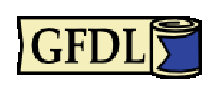
\includegraphics[width=1cm]{gfdl-logo-small.eps}
        \fi

Copyright (c) 2012  Laurent Claessens

Permission is granted to copy, distribute and/or modify this document under the terms of the \href{http://www.gnu.org/licenses/fdl-1.3.html}{GNU Free Documentation License}, Version 1.3 or any later version published by the Free Software Foundation; with no Invariant Sections, no Front-Cover Texts, and no Back-Cover Texts. A copy of the license is included in the chapter entitled ``GNU Free Documentation~License''.

\vspace{0.5cm}

Vous avez le droit de copier, distribuer et modifier ce document pourvu que vous suiviez les règles de la \wikipedia{fr}{GFDL}{GNU Free Documentation License}.

\end{center}
